%%----------------------------------------------------------------------------
%% Onderzoekstechnieken: De centrale limietstelling
%%----------------------------------------------------------------------------

\documentclass[aspectratio=169]{beamer}

%==============================================================================
% Aanloop
%==============================================================================

%---------- Vormgeving --------------------------------------------------------

\usetheme{hogent}

\usecolortheme{hgwhite} % witte achtergrond, zwarte tekst

\usepackage{graphicx,multicol}
\usepackage{comment,enumerate,hyperref}
\usepackage{amsmath,amsfonts,amssymb}
\usepackage[dutch]{babel}
\usepackage{multirow}
\usepackage{eurosym}
\usepackage{listings}
\usepackage{textcomp}
\usepackage{framed}
\usepackage{wrapfig}
\usepackage{tabu} %needed for \tabulinesep
\usepackage{wrapfig}
\usepackage{pgf-pie}
\usepackage{pgfplots}

%---------- Configuratie ------------------------------------------------------

\pgfplotsset{compat=1.16}
\usetikzlibrary{arrows,shapes,backgrounds,positioning,shadows}
\usetikzlibrary{pgfplots.statistics}

%---------- Commando-definities -----------------------------------------------

\newcommand{\tabitem}{~~\llap{\textbullet}~~}
\newcommand{\alertbox}[2][hgblue]{%
  \setbeamercolor{alertbox}{bg=#1,fg=white}
  \begin{beamercolorbox}[sep=2pt,center]{alertbox}
    \textbf{#2}
  \end{beamercolorbox}
}

%---------- Info over de presentatie ------------------------------------------

\title{Chapter 4. The Central Limit Theorem}
\subtitle{Research techniques}
\author{Jens Buysse \and Pieter-Jan Maenhaut \and Bert {Van Vreckem}}
\date{AY 2020-2021}

%==============================================================================
% Inhoud presentatie
%==============================================================================

\begin{document}

\begin{frame}
  \maketitle
\end{frame}

\begin{frame}
  \frametitle{What's on the menu?}
  
  \tableofcontents
\end{frame}

\begin{frame}
  \frametitle{Learning Goals}
  
  \begin{itemize}
    \item Probability distribution of a sample
    \item The normal and Student-$t$ distribution
    \item Formulate the central limit theorem and explain its importance for statistical analysis
    \item Calculate confidence intervals
  \end{itemize}
\end{frame}

\section{Probability Distribution of a Sample}

\begin{frame}
  \frametitle{What do you remember from probability theory?}
  
  \begin{columns}
    \column{.5\textwidth}
    \begin{itemize}
      \item Sample space
      \item Outcome
      \item Event
      \item Probability space
    \end{itemize}
    
    \column{.5\textwidth}
    \centering
    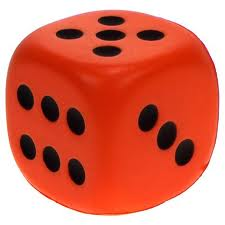
\includegraphics[width=.3\textwidth]{les04-dobbelsteen}
  \end{columns}
  
\end{frame}

\begin{frame}
  \frametitle{Probability Distribution - 1 Dice}
  
  What is the probability of each outcome when rolling a single dice?
  
  \begin{center}
    \begin{tabular}{|c|c|c|c|c|c|}
      \hline
      1&2&3&4&5&6\\
      \hline
      \onslide<2->{$\frac{1}{6}}$ &\onslide<2->{$\frac{1}{6}}$ &\onslide<2->{$\frac{1}{6}}$ &\onslide<2->{$\frac{1}{6}}$ &\onslide<2->{$\frac{1}{6}}$ &     \onslide<2->{$\frac{1}{6}}$ \\
      \hline
      
    \end{tabular}
  \end{center}
  
  \onslide<2->{%
    \begin{center}
      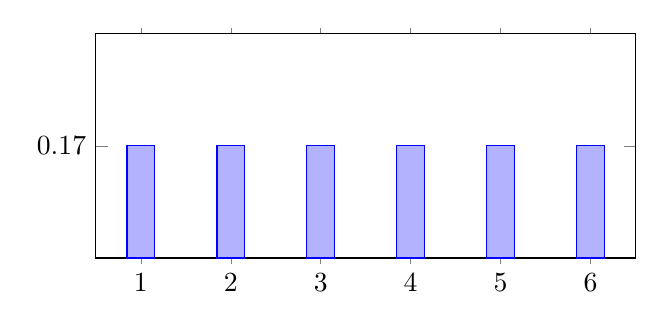
\begin{tikzpicture}
      \begin{axis}[ybar,ytick=data, anchor=north, yscale=.5]
      \addplot
      coordinates {
        (1, 1/6)
        (2, 1/6)
        (3, 1/6)
        (4, 1/6)
        (5, 1/6)
        (6, 1/6)};
      \end{axis}
      \end{tikzpicture}
  \end{center}}
  
\end{frame}

\begin{frame}
  \frametitle{Probability Distribution - 2 Dices}
  
  \begin{center}
    \begin{tabular}{|c|c|c|c|c|c|c|c|c|c|c|c|}
      \hline
      2&3&4&5&6&7&8&9&10&11&12\\
      \hline
      \onslide<2->{$\frac{1}{36}}$ &\onslide<2->{$\frac{2}{36}}$ &\onslide<2->{$\frac{3}{36}}$ &\onslide<2->{$\frac{4}{36}}$ &\onslide<2->{$\frac{5}{36}}$ & \onslide<2->{$\frac{6}{36}}$ & \onslide<2->{$\frac{5}{36}}$ &\onslide<2->{$\frac{4}{36}}$ & \onslide<2->{$\frac{3}{36}}$ &\onslide<2->{$\frac{2}{36}}$ &\onslide<2->{$\frac{1}{36}}$ \\
      \hline
      
    \end{tabular}
  \end{center}
  
  \onslide<2->{%
    \begin{center}
      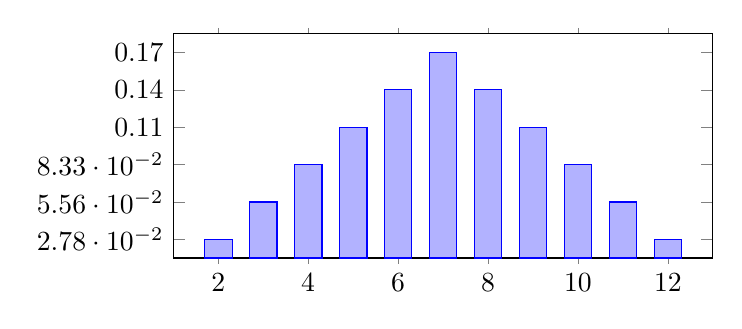
\begin{tikzpicture}
      \begin{axis}[ybar,ytick=data, anchor=north, yscale=.5]
      \addplot
      coordinates {
        (2, 1/36)
        (3, 2/36)
        (4, 3/36)
        (5, 4/36)
        (6, 5/36)
        (7, 6/36)
        (8, 5/36)
        (9, 4/36)
        (10, 3/36)
        (11, 2/36)
        (12, 1/36)
      };
      
      \end{axis}
      \end{tikzpicture}
    \end{center}
  }
  
\end{frame}

\pgfmathdeclarefunction{gauss}{2}{%
  \pgfmathparse{1/(#2*sqrt(2*pi))*exp(-((x-#1)^2)/(2*#2^2))}%
}

\begin{frame}
  \frametitle{Continuous Probability Distr.}
  
  The reaction speed $x$ of Superman (in ms) can be represented as follows:
  
  \bigskip
  
  \begin{columns}
    \begin{column}{.85\textwidth}
      \begin{tikzpicture}
        \begin{axis}[
          domain=0:10, samples=100,
          axis lines*=left, xlabel=$x$ (ms), ylabel=$y$,
          every axis y label/.style={at=(current axis.above origin),anchor=south},
          every axis x label/.style={at=(current axis.right of origin),anchor=west},
          height=5cm, width=11cm,
          xtick={5,3.5,6.5}, ytick=\empty,
          enlargelimits=false, clip=false, axis on top,
          grid = major
          ]
          \addplot [fill=cyan!20, draw=none, domain=0:9] {gauss(5,1.5)} \closedcycle;
          \draw [yshift=-0.6cm, latex-latex](axis cs:3.5,0) -- node [fill=white] {$\sigma$} (axis cs:4.99,0);
          \draw [yshift=-0.6cm, latex-latex](axis cs:5.01,0) -- node [fill=white] {$\sigma$} (axis cs:6.5,0);
          \draw [-](axis cs:5,-0.035) -- (axis cs:5,-0.06);
          \node at (axis cs:5,-0.075) {$\mu$};
        \end{axis}
      \end{tikzpicture}
    \end{column}
    \begin{column}{.15\textwidth}
      
\includegraphics[width=1.5cm]{les2-hero-3}
    \end{column}
  \end{columns}
  
\end{frame}

\begin{frame}
  \frametitle{\textit{Standard} Normal Distribution}
  
  \begin{columns}[c]
    \column{.5\textwidth}
    normal distribution
    $x \in X \sim Nor(\mu, \sigma)$
    \begin{tikzpicture}
    \begin{axis}[
    domain=-2.5:2.5,
    axis lines*=left,
    xmin=-2.5, xmax=2.5,
    ymin=0, ymax=0.39,
    xlabel=$X$,
    every axis x label/.style={at=(current axis.right of origin),anchor=west},
    every axis y label/.style={at=(current axis.above origin),anchor=south},
    height=4cm, width=6cm,
    xtick={-1.4,0,1.4},
    xticklabels={$\mu-\sigma$,$\mu$,$\mu+\sigma$},
    ytick=\empty,
    enlargelimits=false,
    axis on top,
    clip=false,
    ]
    \addplot[very thick,smooth,draw=hgblue]{gauss(0,1.4)};
    \draw [-](axis cs:0.4,0) -- (axis cs:0.4,0.274); %vertical line
    \node at (axis cs: 0.56,0.1) {$x$}; %label x
    \draw [latex-latex](axis cs:2.2,0.22) -- (axis cs:3.5,0.22);
    \end{axis}
    \end{tikzpicture}
    \column{.5\textwidth}
    \textbf{standard} normal distribution
    $z \in Z \sim Nor(0, 1)$
    \begin{tikzpicture}
    \begin{axis}[
    domain=-2.5:2.5,
    axis lines*=left,
    xmin=-2.5, xmax=2.5,
    ymin=0, ymax=0.39,
    xlabel=$Z$,
    every axis x label/.style={at=(current axis.right of origin),anchor=west},
    every axis y label/.style={at=(current axis.above origin),anchor=south},
    height=4cm, width=6cm,
    xtick={-1,0,1},
    enlargelimits=false,
    axis on top,
    clip=false,
    ]
    \addplot[very thick,smooth,draw=hgblue]{gauss(0,1)};
    \draw [-](axis cs:0.286,0) -- (axis cs:0.286,0.383); %vertical line
    \node at (axis cs: 0.42,0.12 ) {$z$}; %label z
    \end{axis}
    \end{tikzpicture}
  \end{columns}
  \vfill
  $x$ and $z$ have a similar position on the Gaussian bell curve.\\
  What is the mathematical relationship between $x$ and $z$?
  \vfill
  \pause
  {\Large $x = \mu + z . \sigma$} ~~~ and ~~~ {\Large $z = \frac{x - \mu}{\sigma}$}
\end{frame}

\begin{frame}
  \frametitle{Standard Normal Distribution}
  
  % Bron: http://johncanning.net/wp/?p=1202
  \begin{center}
    \begin{tikzpicture}
    \begin{axis}[
    no markers, domain=0:10, samples=100,
    axis lines*=left,height=6cm, width=10cm,
    xtick={-3, -2, -1, 0, 1, 2, 3}, ytick=\empty,
    enlargelimits=false, clip=false, axis on top,
    grid = major
    ]
    \addplot [smooth,fill=cyan!20, draw=none, domain=-3:3] {gauss(0,1)} \closedcycle;
    \addplot [smooth,fill=orange!20, draw=none, domain=-3:-2] {gauss(0,1)} \closedcycle;
    \addplot [smooth,fill=orange!20, draw=none, domain=2:3] {gauss(0,1)} \closedcycle;
    \addplot [smooth,fill=blue!20, draw=none, domain=-2:-1] {gauss(0,1)} \closedcycle;
    \addplot [smooth,fill=blue!20, draw=none, domain=1:2] {gauss(0,1)} \closedcycle;
    \addplot[<->] coordinates {(-1,0.4) (1,0.4)};
    \addplot[<->] coordinates {(-2,0.3) (2,0.3)};
    \addplot[<->] coordinates {(-3,0.2) (3,0.2)};
    \node[coordinate, pin={68.3\%}] at (axis cs: 0, 0.35){};
    \node[coordinate, pin={95.4\%}] at (axis cs: 0, 0.25){};
    \node[coordinate, pin={99.7\%}] at (axis cs: 0, 0.15){};
    \node[coordinate, pin={34.1\%}] at (axis cs: -0.5, 0){};
    \node[coordinate, pin={34.1\%}] at (axis cs: 0.5, 0){};
    \node[coordinate, pin={13.6\%}] at (axis cs: 1.5, 0){};
    \node[coordinate, pin={13.6\%}] at (axis cs: -1.5, 0){};
    \node[coordinate, pin={2.1\%}] at (axis cs: 2.5, 0){};
    \node[coordinate, pin={2.1\%}] at (axis cs: -2.5, 0){};
    \end{axis}
    \end{tikzpicture}
  \end{center}
\end{frame}

\begin{frame}[fragile]
  \frametitle{Main Functions in R}
  
  For a normal distribution with mean \texttt{m} and standard deviation \texttt{s}:
  \vfill
  \centering
  \begin{tabular}{ll}
    \textbf{Functie}      & \textbf{Betekenis}                          \\ \hline
    \verb|pnorm(x, m, s)| & Left tail probability, $P(X<\mathtt{x})$         \\
    \verb|dnorm(x, m, s)| & Altitude of the Gaussian curve at point \texttt{x} \\
    \verb|qnorm(p, m, s)| & What boundary value contains \texttt{p}\%   \\
    & of the observations?                        \\
    \verb|rnorm(n, m, s)| & Generate \texttt{n} normally distributed random numbers
  \end{tabular}
  \vfill
  If the values for arguments \texttt{m} and \texttt{s} are omitted, the standard normal distribution is used: \texttt{pnorm(x)=pnorm(x,0,1)}
\end{frame}

\begin{frame}
  \frametitle{Calculating Probabilities}
  What is the probability that \dots\\
  \dots Superman's reaction speed is over 6 ms?
  \vfill
  Mathematical Notation:\\
  \hspace{1cm}$P( X > 6)$ = ?\hspace{1cm}met $X \sim Nor(\mu=5,\sigma=1,5)$
  \vfill
  \begin{center}
    \begin{tikzpicture}
    \begin{axis}[
    domain=0:10,
    axis lines*=left,
    xlabel=$x$,
    every axis x label/.style={at=(current axis.right of origin),anchor=west},
    every axis y label/.style={at=(current axis.above origin),anchor=south},
    height=5cm, width=8cm,
    xtick={3.5,5,6.5},
    ytick=\empty,
    enlargelimits=false,
    axis on top,
    clip=false,
    ]
    \addplot[fill=cyan!20, draw=black, domain=6:10] {gauss(5,1.5)} \closedcycle;
    \addplot[very thick,smooth,draw=hgblue]{gauss(5,1.5)};
    \draw [-latex](axis cs:7,0.05) -- (axis cs:8.5,0.1);
    \node at (axis cs: 10, 0.1) {$P(X>6)$};
    \draw [-](axis cs:6,-0.005) -- (axis cs:6,-0.040);
    \node at (axis cs: 6, -0.055) {$6$};
    \end{axis}
    \end{tikzpicture}
  \end{center}
\end{frame}

\begin{frame}
  \frametitle{Calculating Probabilities: $z$-table}
  
  $P( X > 6)$ = ?\hspace{1cm}with $X \sim Nor(\mu=5,\sigma=1,5)$
  
  \bigskip
  
  (Old) calculation method using z-table, e.g.
  
  \url{http://sixsigmastudyguide.com/wp-content/uploads/2014/04/z-table.jpg}
  
  \begin{enumerate}
    \pause
    \item Calculate the $z$-score\\
    $z=\frac{6-5}{1,5}=0,667$ so $P(X>6) = P(Z>0,667)$
    \item Convert to a \textbf{\textit{left}} tail probability
    \begin{itemize}
      \item 100\% probability rule: $P(Z>0,667)=1-P(Z<0,667)$
      \item or symmetry rule: $P(Z>0,667)=P(Z<-0,667)$
    \end{itemize}
    \item look for the corresponding value in the $z$-table\\
  \end{enumerate}
\end{frame}

\begin{frame}
  \frametitle{Calculating Probabilities: using R}
  
  $P( X > 6)$ = ?\hspace{1cm}with $X \sim Nor(\mu=5,\sigma=1,5)$
  
  Calculated directly using R (or using a calculator)
  
  \begin{itemize}
    \pause
    \item first convert to a \textbf{\textit{left}} tail probability:\\
    using 100\% probability rule: $P(X>6)=1-P(X<6)$
    \item calculate using R: $1-P(X<6)=$\texttt{1-pnorm(6,5,1.5)}
  \end{itemize}
\end{frame}

\begin{frame}
  \frametitle{Examples}
  
  \begin{enumerate}
    \item What is the probability that Superman reacts in less than 4 ms?
    \item What is the probability that he reacts in less than 7 ms?
    \item What is the probability that he reacts in less than 3 ms?
    \item What is the probability that he reacts between 2 en 6.5 ms?
    \item What interval contains 80\% of his reaction speed?
  \end{enumerate}
\end{frame}

\begin{frame}
  \frametitle{Question 3: $P(X<3)$}
  
  \begin{center}
    \begin{tikzpicture}
    \begin{axis}[no markers,domain=-4:4,axis lines*=left,yscale=.7,enlargelimits=false,clip=false]
    \addplot[very thick,smooth,draw=hgblue]{gauss(0, 1)};
    \addplot[smooth,fill=black!20, draw=black, domain=-4:-4/3] {gauss(0,1)} \closedcycle;
    
    \node at (axis cs: -1.33, -.05) {\small -1.33};
    \end{axis}
    \end{tikzpicture}
  \end{center}
\end{frame}

\begin{frame}
  \frametitle{Question 4: $P(2<X<6,5)$}
  
  \begin{center}
    \begin{tikzpicture}
    \begin{axis}[no markers,domain=-4:4,axis lines*=left,yscale=.7,enlargelimits=false,clip=false]
    \addplot[very thick,smooth,draw=hgblue]{gauss(0, 1)};
    \addplot[smooth,fill=black!20, draw=black, domain=-2:1] {gauss(0,1)} \closedcycle;
    
    \node at (axis cs: 1, -.05) {\small 1};
    \end{axis}
    \end{tikzpicture}
  \end{center}
\end{frame}

\begin{frame}
  \frametitle{Question 5}
  
  For what value of $x$ is $P(X<x) = 80\%$?
  
  \vfill
  
  \begin{center}
    \begin{tikzpicture}
    \begin{axis}[no markers,domain=-4:4,axis lines*=left,yscale=.7,enlargelimits=false,clip=false]
    \addplot[very thick,smooth,draw=hgblue]{gauss(0, 1)};
    \addplot[smooth,fill=black!20, draw=black, domain=-4:.84] {gauss(0,1)} \closedcycle;
    
    \node at (axis cs: .84, -.05) {\small .84};
    \end{axis}
    \end{tikzpicture}
  \end{center}
\end{frame}

\section{The Central Limit Theorem}

\begin{frame}
  \frametitle{The Central Limit Theorem}
  
  \alertbox{If the size of the sample is sufficiently large, the probability distribution of the sample mean will approximate a normal distribution, regardless of the probability distribution of the underlying population.}
  
  \vfill
  
  \begin{columns}[c]
    \column{.33\textwidth}
    
\includegraphics[width=2cm]{les4-centrlimiet}
    \column{.33\textwidth}
    \begin{itemize}
      \item 1 test
      \item 25 tests
      \item 100 tests
    \end{itemize}
    \column{.33\textwidth}
    
\includegraphics[width=2cm]{les2-hero-3}
  \end{columns}
  
  \vfill
  Demo: \url{https://students.brown.edu/seeing-theory/probability-distributions/index.html}
\end{frame}

\begin{frame}
  \frametitle{The Central Limit Theorem}
  Consider a random sample of $n$ observations drawn from a population with expected value $\mu$ and standard deviation $\sigma$.
  If $n$ is sufficiently large, the probability distribution of the sample mean $\overline{x}$ will approximate a 
  normal distribution with mean $\mu_{\overline{x}} = \mu$ and standard deviation $\sigma_{\overline{x}} = \frac{\sigma}{\sqrt{n}}$.

  \vspace{0.4cm}
  The larger the sample, the better the probability distribution of $\overline{x}$ will approximate the expected value of the population, $\mu$.
\end{frame}

\section{From Sample to Population}

\begin{frame}
  \frametitle{Point Estimate}
  \alertbox{A \textcolor{hgyellow}{Point Estimate} for a population parameter is a formula or equation that allows us to calculate a value to estimate that parameter.}
\end{frame}

\subsection{Confidence Interval}
\begin{frame}
  \frametitle{Confidence Interval}
  \alertbox{A \textcolor{hgyellow}{confidence interval} is an equation or formula that allows us to construct an 
  interval that will contain the parameter to be estimated with a certain \textcolor{hgyellow}{level of confidence}.}
\end{frame}

\subsection{Confidence Interval for a Large Sample}

\begin{frame}
  \frametitle{Conf. Int. - Large Sample}

  Given a sample with mean $\overline{x}$.\\
  We are looking for an interval $\left[ ~\overline{x}-b~,~\overline{x}+b~\right]$ for which we can say with a level of confidence $(1-\alpha)$ of for example 95\% that $\mu$ is inside this interval.
  \vfill
  \[ P\left( \overline{x}-b < \mu < \overline{x}+b \right) = 1-\alpha = 0,95 \]
  \vfill
  \begin{center}
    \begin{tikzpicture}[scale=.8]
    \begin{axis}[
    domain=-3:3,
    axis lines*=left,
    height=5cm, width=12cm,
    xtick={-1.96,0,1.96},
    xticklabels={$\overline{x}-b$,$\overline{x}$,$\overline{x}+b$},
    ytick=\empty,
    enlargelimits=false,
    axis on top,
    clip=false,
    ]
    \addplot[fill=cyan!20, draw=black, domain=-1.96:1.96] {gauss(0,1)} \closedcycle;
    \addplot[very thick,smooth,draw=hgblue]{gauss(0,1)};
    %\addplot[smooth,dashed,draw=hgblue]{gauss(0.8,1)};
    \node [text width=1.5cm,fill=cyan!20,align=center] at (axis cs: 0, 0.17) {95\%\\($1-\alpha$)};
    \draw [-latex](axis cs:2.15,0.02) -- (axis cs:2.4,0.07);
    \node [text width=1cm,fill=white,align=center] at (axis cs: 2.5,0.14) {2,5\%\\($\frac{\alpha}{2}$)};
    \draw [-latex](axis cs:-2.15,0.02) -- (axis cs:-2.3,0.07);
    \node [text width=1cm,align=center] at (axis cs: -2.3,0.14) {2,5\%\\($\frac{\alpha}{2}$)};
    \draw [-](axis cs:0.6,0.02) -- (axis cs:0.6,-0.06);
    \node [align=center] at (axis cs: 0.6,-0.09) {$\mu$};
    \end{axis}
    \end{tikzpicture}
  \end{center}
\end{frame}

\begin{frame}
  \frametitle{Conf. Int. - Large Sample}
  
  Because of the central limit theorem we know that:
  $\overline{x} \in \overline{X} \sim Nor(\mu,\frac{\sigma}{\sqrt{n}})$
  
  And because of the symmetry we can say:
  \[ P\left( \overline{x}-b < \mu < \overline{x}-b \right) = P\left( \mu-b < \overline{x} < \mu+b \right) \]
  
  \vfill
  
  \begin{center}
    \begin{tikzpicture}[scale=.8]
    
    \begin{axis}[
    domain=-3:3,
    axis lines*=left,
    height=5cm, width=12cm,
    xlabel=$\overline{X}$,
    every axis x label/.style={at=(current axis.right of origin),anchor=west},
    every axis y label/.style={at=(current axis.above origin),anchor=south},
    xtick={-1.36,-0.4,0.6,1.6,2.56},
    xticklabels={$\mu-b$,,$\mu$,,$\mu+b$},
    ytick=\empty,
    enlargelimits=false,
    axis on top,
    clip=false,
    ]
    \addplot[fill=cyan!20, draw=black, domain=-1.36:2.56] {gauss(0.6,1)} \closedcycle;
    \addplot[very thick,smooth,draw=hgblue]{gauss(0.6,1)};
    \addplot[smooth,dashed,draw=hgblue]{gauss(0,1)};
    \node [text width=1.5cm,align=center] at (axis cs: 0.6, 0.17) {95\%\\($1-\alpha$)};
    \draw [-latex](axis cs:2.75,0.02) -- (axis cs:3.0,0.07);
    \node [text width=1cm,fill=white,align=center] at (axis cs: 3.1,0.14) {2,5\%\\($\frac{\alpha}{2}$)};
    \draw [-latex](axis cs:-1.55,0.02) -- (axis cs:-1.7,0.07);
    \node [text width=0.8cm,fill=white,align=center] at (axis cs: -1.8,0.14) {2,5\%\\($\frac{\alpha}{2}$)};
    \draw [-,dashed](axis cs:0,0.4) -- (axis cs:0,-0.07);
    \node [align=center] at (axis cs: 0,-0.1) {$\overline{x}$};
    \draw [latex-latex](axis cs:0.6,-0.07) -- node [fill=white] {$\frac{\sigma}{\sqrt{n}}$} (axis cs:1.6,-0.07);
    \end{axis}
    \end{tikzpicture}
  \end{center}
  
\end{frame}

\begin{frame}
  \frametitle{Conf. Int. - Large Sample}
  
  \bigskip
  
  We now calculate the $z$-score for $\overline{x}$:
  $z = \frac{\overline{x} - \mu}{\frac{\sigma}{\sqrt{n}}}$
  
  We lookup (or calculate) the value $z_\frac{\alpha}{2}$ for which:
  \[ P\left(-z_{\frac{\alpha}{2}} < z < z_{\frac{\alpha}{2}}\right) = 1 - \alpha = 0.95 \]
  \[ P\left(z < z_{\frac{\alpha}{2}}\right) = 1 - \frac{\alpha}{2} = 0.975 \]
  \[ z_{\frac{\alpha}{2}} = \texttt{qnorm(0.975)} \approx 1.96 \]
  
  \vfill
  
  
  \begin{center}
    \begin{tikzpicture}[scale=.8]
    \begin{axis}[
    domain=-3:3,
    axis lines*=left,
    xlabel=$Z$,
    every axis x label/.style={at=(current axis.right of origin),anchor=west},
    every axis y label/.style={at=(current axis.above origin),anchor=south},
    height=4cm, width=10cm,
    xtick={-1.96,-1,0,1,1.96},
    xticklabels={-$z_\frac{\alpha}{2}$,-1,0,1,$z_\frac{\alpha}{2}$},
    ytick=\empty,
    enlargelimits=false,
    axis on top,
    clip=false,
    ]
    \addplot[fill=cyan!20, draw=black, domain=-1.96:1.96] {gauss(0,1)} \closedcycle;
    \addplot[very thick,smooth,draw=hgblue]{gauss(0,1)};
    \node [text width=1.5cm,align=center] at (axis cs: 0, 0.15) {95\%\\($1-\alpha$)};
    \draw [-latex](axis cs:2.15,0.02) -- (axis cs:2.4,0.07);
    \node [text width=1cm,align=center] at (axis cs: 2.5,0.16) {2,5\%\\($\frac{\alpha}{2}$)};
    \draw [-latex](axis cs:-2.15,0.02) -- (axis cs:-2.3,0.07);
    \node [text width=1cm,align=center] at (axis cs: -2.3,0.16) {2,5\%\\($\frac{\alpha}{2}$)};
    
    \end{axis}
    \end{tikzpicture}
  \end{center}
  
\end{frame}

\begin{frame}
  \frametitle{Conf. Int. - Large Sample}
  
  The result is:
  \[ P\left(-1,96 < \frac{\overline{x} - \mu}{\frac{\sigma}{\sqrt{n}}} < 1,96 \right) = 0,95 \]
  \[ P\left( \mu-1,96 \frac{\sigma}{\sqrt{n}} < \overline{x} < \mu+1,96 \frac{\sigma}{\sqrt{n}} \right)  = 0,95 \]
  
  Because of symmetry we can swap $\mu$ and $\overline{x}$:
  \[ P\left( \overline{x}-1,96 \frac{\sigma}{\sqrt{n}} < \mu < \overline{x}+1,96 \frac{\sigma}{\sqrt{n}} \right)  = 0,95 \]
  
  Now we can say with 95\% confidence that:
  \[ \mu \in \left[~\overline{x}-1,96.\frac{\sigma}{\sqrt{n}}~,~\overline{x}+1,96. \frac{\sigma}{\sqrt{n}}~\right] \]
  
  \small (in practice we will use $s_{sample}$ as an estimate for $\sigma_{population}$)
  
\end{frame}

\subsection{Confidence Interval for a Small Sample}

\begin{frame}
  \frametitle{Conf. Int. - Small Sample}
  For a \textit{\textbf{small}} sample the central limit theorem is \textbf{no longer} valid.
  \vfill
  Instead we can say:\\
  \vfill
  If a population $X$ has a normal distribution $(X \sim Nor(\mu,\sigma))$
  and you take a \textit{small} sample with mean $\overline{x}$ and standard deviation $s$, 
  then
  \[ t = \frac{\overline{x} - \mu}{\frac{s}{\sqrt{n}}} \]
  will behave as a t-distribution with ~$n-1$~ degrees of freedom
  
\end{frame}

\begin{frame}
  \frametitle{Student t-distribution for \textit{small} samples}
  \bigskip
  \centering
  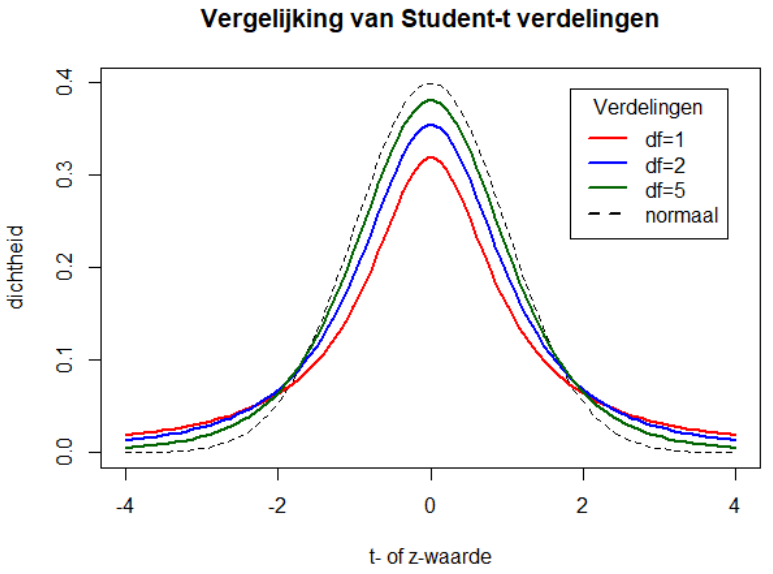
\includegraphics[height=.9\textheight]{les04-t-distrib}
\end{frame}

\begin{frame}
  \frametitle{Student $t$-distribution in R}
  
  For a $t$-distribution with ~\texttt{df}~ degrees of freedom:
  
  \small (\texttt{df = degrees of freedom})
  \vfill
  \centering
  \begin{tabular}{ll}
    \textbf{Function}  & \textbf{Return Value}                       \\
    \hline
    \texttt{pt(x, df)} & Left tail probability, $P(X<\mathtt{x})$    \\
    \texttt{dt(x, df)} & Height of the curve at point \texttt{x}     \\
    \texttt{qt(p, df)} & What boundary value contains \texttt{p}\%   \\
                       & of the observations?                        \\
    \texttt{rt(n, df)} & Generate \texttt{n} random numbers using this distribution \\
  \end{tabular}
  
\end{frame}

\begin{frame}
  \frametitle{Conf. Int. - Small Sample}
  To determine the confidence interval for the mean $\mu$ of a population, based on a \textit{small} sample, we first calculate $t_ {\frac{\alpha}{2},df}$.
  
  \vfill
  With a confidence level of 95\% we have $\frac{\alpha}{2}=0,025$\\
  Assume for example $n=5$ (so \texttt{df=4}), then we have
  \[ t_ {\frac{\alpha}{2},df} = \texttt{qt(0.975,4)} = 2.776 \]
  
  \vfill
  We can say with a certainty of 95\% that:
  \[ \mu \in \left[~ \overline{x} - t_{\frac{\alpha}{2},df}.\frac{s}{\sqrt{n}} ~,~ \overline{x} + t_{\frac{\alpha}{2},df}.\frac{s}{\sqrt{n}} ~\right] \]
  
\end{frame}


\subsection{Confidence Interval for a Fraction}

\begin{frame}
  \frametitle{Conf. Int. - Fraction}
  \[ \overline{p} = \frac{\textnormal{number of successes}}{n} \]
  \begin{itemize}
    \item The expected probability distribution of $\overline{p}$ is $p$.
    \item The standard deviation of the probability distribution of $\overline{p}$ is $\sqrt{\frac{pq}{n}}$
    \item For large samples, $\overline{p}$ is approximately normally distributed
  \end{itemize}

  Since $\overline{p}$ is a sample mean of the number of successes, we can calculate a confidence interval analogous to the previously discussed interval estimate of $\mu$ for large samples.
  
  \[ \overline{p} \pm z_{\frac{\alpha}{2}}.\sqrt{\frac{\overline{p}\overline{q}}{n}} \]
  with $\overline{p} = \frac{x}{n}$ en $\overline{q} = 1- \overline{p}$
  
\end{frame}


\end{document}